\documentclass{article}

% ============================================================
% INFR11269 Machine Learning Systems — Coursework Report
% Academic year 2026/27
%
% This coursework uses the official ICLR 2027 LaTeX style.
%
% IMPORTANT FORMAT RULES
% - Do not edit iclr2027_conference.sty.
% - Do not change page geometry, text width/height, base font size,
%   or line spacing.
% - Do not enable \iclrfinalcopy.
% - Normal content packages are fine if they do not alter the report format.
%
% Main-body page limit: six pages.
% References and Appendix do NOT count toward the main-body page limit.
% Reviewers are not obliged to read Appendix at all. Please put your main content
% in the main body.
%
% AI policy:
% Academic integrity is an underlying principle of research and academic practice.
% All submitted work is expected to be your own, including any material you have
% generated yourself with the assistance of AI tools such as ELM, ChatGPT,
% Bing Chat, Claude, Google Gemini, or any other automated assistance.
% For all such material you must make prominent explicit acknowledgement and
% explain clearly what you have done in the AI declaration section.
% This includes using AI to directly generate text, code, figures or similar
% or to complete other tasks. In all cases, you remain entirely responsible
% for the material you produce.
% ============================================================

\usepackage{iclr2027_conference,times}

\usepackage{hyperref}
\usepackage{url}
\usepackage{booktabs}
\usepackage{graphicx}
\usepackage{amsmath}
\usepackage{amssymb}
\usepackage{pgfplots}
\pgfplotsset{compat=1.18}

% The official ICLR archive includes math_commands.tex. It is optional:
%%%%% NEW MATH DEFINITIONS %%%%%

\usepackage{amsmath,amsfonts,bm}

% Mark sections of captions for referring to divisions of figures
\newcommand{\figleft}{{\em (Left)}}
\newcommand{\figcenter}{{\em (Center)}}
\newcommand{\figright}{{\em (Right)}}
\newcommand{\figtop}{{\em (Top)}}
\newcommand{\figbottom}{{\em (Bottom)}}
\newcommand{\captiona}{{\em (a)}}
\newcommand{\captionb}{{\em (b)}}
\newcommand{\captionc}{{\em (c)}}
\newcommand{\captiond}{{\em (d)}}

% Highlight a newly defined term
\newcommand{\newterm}[1]{{\bf #1}}


% Figure reference, lower-case.
\def\figref#1{figure~\ref{#1}}
% Figure reference, capital. For start of sentence
\def\Figref#1{Figure~\ref{#1}}
\def\twofigref#1#2{figures \ref{#1} and \ref{#2}}
\def\quadfigref#1#2#3#4{figures \ref{#1}, \ref{#2}, \ref{#3} and \ref{#4}}
% Section reference, lower-case.
\def\secref#1{section~\ref{#1}}
% Section reference, capital.
\def\Secref#1{Section~\ref{#1}}
% Reference to two sections.
\def\twosecrefs#1#2{sections \ref{#1} and \ref{#2}}
% Reference to three sections.
\def\secrefs#1#2#3{sections \ref{#1}, \ref{#2} and \ref{#3}}
% Reference to an equation, lower-case.
\def\eqref#1{equation~\ref{#1}}
% Reference to an equation, upper case
\def\Eqref#1{Equation~\ref{#1}}
% A raw reference to an equation---avoid using if possible
\def\plaineqref#1{\ref{#1}}
% Reference to a chapter, lower-case.
\def\chapref#1{chapter~\ref{#1}}
% Reference to an equation, upper case.
\def\Chapref#1{Chapter~\ref{#1}}
% Reference to a range of chapters
\def\rangechapref#1#2{chapters\ref{#1}--\ref{#2}}
% Reference to an algorithm, lower-case.
\def\algref#1{algorithm~\ref{#1}}
% Reference to an algorithm, upper case.
\def\Algref#1{Algorithm~\ref{#1}}
\def\twoalgref#1#2{algorithms \ref{#1} and \ref{#2}}
\def\Twoalgref#1#2{Algorithms \ref{#1} and \ref{#2}}
% Reference to a part, lower case
\def\partref#1{part~\ref{#1}}
% Reference to a part, upper case
\def\Partref#1{Part~\ref{#1}}
\def\twopartref#1#2{parts \ref{#1} and \ref{#2}}

\def\ceil#1{\lceil #1 \rceil}
\def\floor#1{\lfloor #1 \rfloor}
\def\1{\bm{1}}
\newcommand{\train}{\mathcal{D}}
\newcommand{\valid}{\mathcal{D_{\mathrm{valid}}}}
\newcommand{\test}{\mathcal{D_{\mathrm{test}}}}

\def\eps{{\epsilon}}


% Random variables
\def\reta{{\textnormal{$\eta$}}}
\def\ra{{\textnormal{a}}}
\def\rb{{\textnormal{b}}}
\def\rc{{\textnormal{c}}}
\def\rd{{\textnormal{d}}}
\def\re{{\textnormal{e}}}
\def\rf{{\textnormal{f}}}
\def\rg{{\textnormal{g}}}
\def\rh{{\textnormal{h}}}
\def\ri{{\textnormal{i}}}
\def\rj{{\textnormal{j}}}
\def\rk{{\textnormal{k}}}
\def\rl{{\textnormal{l}}}
% rm is already a command, just don't name any random variables m
\def\rn{{\textnormal{n}}}
\def\ro{{\textnormal{o}}}
\def\rp{{\textnormal{p}}}
\def\rq{{\textnormal{q}}}
\def\rr{{\textnormal{r}}}
\def\rs{{\textnormal{s}}}
\def\rt{{\textnormal{t}}}
\def\ru{{\textnormal{u}}}
\def\rv{{\textnormal{v}}}
\def\rw{{\textnormal{w}}}
\def\rx{{\textnormal{x}}}
\def\ry{{\textnormal{y}}}
\def\rz{{\textnormal{z}}}

% Random vectors
\def\rvepsilon{{\mathbf{\epsilon}}}
\def\rvtheta{{\mathbf{\theta}}}
\def\rva{{\mathbf{a}}}
\def\rvb{{\mathbf{b}}}
\def\rvc{{\mathbf{c}}}
\def\rvd{{\mathbf{d}}}
\def\rve{{\mathbf{e}}}
\def\rvf{{\mathbf{f}}}
\def\rvg{{\mathbf{g}}}
\def\rvh{{\mathbf{h}}}
\def\rvu{{\mathbf{i}}}
\def\rvj{{\mathbf{j}}}
\def\rvk{{\mathbf{k}}}
\def\rvl{{\mathbf{l}}}
\def\rvm{{\mathbf{m}}}
\def\rvn{{\mathbf{n}}}
\def\rvo{{\mathbf{o}}}
\def\rvp{{\mathbf{p}}}
\def\rvq{{\mathbf{q}}}
\def\rvr{{\mathbf{r}}}
\def\rvs{{\mathbf{s}}}
\def\rvt{{\mathbf{t}}}
\def\rvu{{\mathbf{u}}}
\def\rvv{{\mathbf{v}}}
\def\rvw{{\mathbf{w}}}
\def\rvx{{\mathbf{x}}}
\def\rvy{{\mathbf{y}}}
\def\rvz{{\mathbf{z}}}

% Elements of random vectors
\def\erva{{\textnormal{a}}}
\def\ervb{{\textnormal{b}}}
\def\ervc{{\textnormal{c}}}
\def\ervd{{\textnormal{d}}}
\def\erve{{\textnormal{e}}}
\def\ervf{{\textnormal{f}}}
\def\ervg{{\textnormal{g}}}
\def\ervh{{\textnormal{h}}}
\def\ervi{{\textnormal{i}}}
\def\ervj{{\textnormal{j}}}
\def\ervk{{\textnormal{k}}}
\def\ervl{{\textnormal{l}}}
\def\ervm{{\textnormal{m}}}
\def\ervn{{\textnormal{n}}}
\def\ervo{{\textnormal{o}}}
\def\ervp{{\textnormal{p}}}
\def\ervq{{\textnormal{q}}}
\def\ervr{{\textnormal{r}}}
\def\ervs{{\textnormal{s}}}
\def\ervt{{\textnormal{t}}}
\def\ervu{{\textnormal{u}}}
\def\ervv{{\textnormal{v}}}
\def\ervw{{\textnormal{w}}}
\def\ervx{{\textnormal{x}}}
\def\ervy{{\textnormal{y}}}
\def\ervz{{\textnormal{z}}}

% Random matrices
\def\rmA{{\mathbf{A}}}
\def\rmB{{\mathbf{B}}}
\def\rmC{{\mathbf{C}}}
\def\rmD{{\mathbf{D}}}
\def\rmE{{\mathbf{E}}}
\def\rmF{{\mathbf{F}}}
\def\rmG{{\mathbf{G}}}
\def\rmH{{\mathbf{H}}}
\def\rmI{{\mathbf{I}}}
\def\rmJ{{\mathbf{J}}}
\def\rmK{{\mathbf{K}}}
\def\rmL{{\mathbf{L}}}
\def\rmM{{\mathbf{M}}}
\def\rmN{{\mathbf{N}}}
\def\rmO{{\mathbf{O}}}
\def\rmP{{\mathbf{P}}}
\def\rmQ{{\mathbf{Q}}}
\def\rmR{{\mathbf{R}}}
\def\rmS{{\mathbf{S}}}
\def\rmT{{\mathbf{T}}}
\def\rmU{{\mathbf{U}}}
\def\rmV{{\mathbf{V}}}
\def\rmW{{\mathbf{W}}}
\def\rmX{{\mathbf{X}}}
\def\rmY{{\mathbf{Y}}}
\def\rmZ{{\mathbf{Z}}}

% Elements of random matrices
\def\ermA{{\textnormal{A}}}
\def\ermB{{\textnormal{B}}}
\def\ermC{{\textnormal{C}}}
\def\ermD{{\textnormal{D}}}
\def\ermE{{\textnormal{E}}}
\def\ermF{{\textnormal{F}}}
\def\ermG{{\textnormal{G}}}
\def\ermH{{\textnormal{H}}}
\def\ermI{{\textnormal{I}}}
\def\ermJ{{\textnormal{J}}}
\def\ermK{{\textnormal{K}}}
\def\ermL{{\textnormal{L}}}
\def\ermM{{\textnormal{M}}}
\def\ermN{{\textnormal{N}}}
\def\ermO{{\textnormal{O}}}
\def\ermP{{\textnormal{P}}}
\def\ermQ{{\textnormal{Q}}}
\def\ermR{{\textnormal{R}}}
\def\ermS{{\textnormal{S}}}
\def\ermT{{\textnormal{T}}}
\def\ermU{{\textnormal{U}}}
\def\ermV{{\textnormal{V}}}
\def\ermW{{\textnormal{W}}}
\def\ermX{{\textnormal{X}}}
\def\ermY{{\textnormal{Y}}}
\def\ermZ{{\textnormal{Z}}}

% Vectors
\def\vzero{{\bm{0}}}
\def\vone{{\bm{1}}}
\def\vmu{{\bm{\mu}}}
\def\vtheta{{\bm{\theta}}}
\def\va{{\bm{a}}}
\def\vb{{\bm{b}}}
\def\vc{{\bm{c}}}
\def\vd{{\bm{d}}}
\def\ve{{\bm{e}}}
\def\vf{{\bm{f}}}
\def\vg{{\bm{g}}}
\def\vh{{\bm{h}}}
\def\vi{{\bm{i}}}
\def\vj{{\bm{j}}}
\def\vk{{\bm{k}}}
\def\vl{{\bm{l}}}
\def\vm{{\bm{m}}}
\def\vn{{\bm{n}}}
\def\vo{{\bm{o}}}
\def\vp{{\bm{p}}}
\def\vq{{\bm{q}}}
\def\vr{{\bm{r}}}
\def\vs{{\bm{s}}}
\def\vt{{\bm{t}}}
\def\vu{{\bm{u}}}
\def\vv{{\bm{v}}}
\def\vw{{\bm{w}}}
\def\vx{{\bm{x}}}
\def\vy{{\bm{y}}}
\def\vz{{\bm{z}}}

% Elements of vectors
\def\evalpha{{\alpha}}
\def\evbeta{{\beta}}
\def\evepsilon{{\epsilon}}
\def\evlambda{{\lambda}}
\def\evomega{{\omega}}
\def\evmu{{\mu}}
\def\evpsi{{\psi}}
\def\evsigma{{\sigma}}
\def\evtheta{{\theta}}
\def\eva{{a}}
\def\evb{{b}}
\def\evc{{c}}
\def\evd{{d}}
\def\eve{{e}}
\def\evf{{f}}
\def\evg{{g}}
\def\evh{{h}}
\def\evi{{i}}
\def\evj{{j}}
\def\evk{{k}}
\def\evl{{l}}
\def\evm{{m}}
\def\evn{{n}}
\def\evo{{o}}
\def\evp{{p}}
\def\evq{{q}}
\def\evr{{r}}
\def\evs{{s}}
\def\evt{{t}}
\def\evu{{u}}
\def\evv{{v}}
\def\evw{{w}}
\def\evx{{x}}
\def\evy{{y}}
\def\evz{{z}}

% Matrix
\def\mA{{\bm{A}}}
\def\mB{{\bm{B}}}
\def\mC{{\bm{C}}}
\def\mD{{\bm{D}}}
\def\mE{{\bm{E}}}
\def\mF{{\bm{F}}}
\def\mG{{\bm{G}}}
\def\mH{{\bm{H}}}
\def\mI{{\bm{I}}}
\def\mJ{{\bm{J}}}
\def\mK{{\bm{K}}}
\def\mL{{\bm{L}}}
\def\mM{{\bm{M}}}
\def\mN{{\bm{N}}}
\def\mO{{\bm{O}}}
\def\mP{{\bm{P}}}
\def\mQ{{\bm{Q}}}
\def\mR{{\bm{R}}}
\def\mS{{\bm{S}}}
\def\mT{{\bm{T}}}
\def\mU{{\bm{U}}}
\def\mV{{\bm{V}}}
\def\mW{{\bm{W}}}
\def\mX{{\bm{X}}}
\def\mY{{\bm{Y}}}
\def\mZ{{\bm{Z}}}
\def\mBeta{{\bm{\beta}}}
\def\mPhi{{\bm{\Phi}}}
\def\mLambda{{\bm{\Lambda}}}
\def\mSigma{{\bm{\Sigma}}}

% Tensor
\DeclareMathAlphabet{\mathsfit}{\encodingdefault}{\sfdefault}{m}{sl}
\SetMathAlphabet{\mathsfit}{bold}{\encodingdefault}{\sfdefault}{bx}{n}
\newcommand{\tens}[1]{\bm{\mathsfit{#1}}}
\def\tA{{\tens{A}}}
\def\tB{{\tens{B}}}
\def\tC{{\tens{C}}}
\def\tD{{\tens{D}}}
\def\tE{{\tens{E}}}
\def\tF{{\tens{F}}}
\def\tG{{\tens{G}}}
\def\tH{{\tens{H}}}
\def\tI{{\tens{I}}}
\def\tJ{{\tens{J}}}
\def\tK{{\tens{K}}}
\def\tL{{\tens{L}}}
\def\tM{{\tens{M}}}
\def\tN{{\tens{N}}}
\def\tO{{\tens{O}}}
\def\tP{{\tens{P}}}
\def\tQ{{\tens{Q}}}
\def\tR{{\tens{R}}}
\def\tS{{\tens{S}}}
\def\tT{{\tens{T}}}
\def\tU{{\tens{U}}}
\def\tV{{\tens{V}}}
\def\tW{{\tens{W}}}
\def\tX{{\tens{X}}}
\def\tY{{\tens{Y}}}
\def\tZ{{\tens{Z}}}


% Graph
\def\gA{{\mathcal{A}}}
\def\gB{{\mathcal{B}}}
\def\gC{{\mathcal{C}}}
\def\gD{{\mathcal{D}}}
\def\gE{{\mathcal{E}}}
\def\gF{{\mathcal{F}}}
\def\gG{{\mathcal{G}}}
\def\gH{{\mathcal{H}}}
\def\gI{{\mathcal{I}}}
\def\gJ{{\mathcal{J}}}
\def\gK{{\mathcal{K}}}
\def\gL{{\mathcal{L}}}
\def\gM{{\mathcal{M}}}
\def\gN{{\mathcal{N}}}
\def\gO{{\mathcal{O}}}
\def\gP{{\mathcal{P}}}
\def\gQ{{\mathcal{Q}}}
\def\gR{{\mathcal{R}}}
\def\gS{{\mathcal{S}}}
\def\gT{{\mathcal{T}}}
\def\gU{{\mathcal{U}}}
\def\gV{{\mathcal{V}}}
\def\gW{{\mathcal{W}}}
\def\gX{{\mathcal{X}}}
\def\gY{{\mathcal{Y}}}
\def\gZ{{\mathcal{Z}}}

% Sets
\def\sA{{\mathbb{A}}}
\def\sB{{\mathbb{B}}}
\def\sC{{\mathbb{C}}}
\def\sD{{\mathbb{D}}}
% Don't use a set called E, because this would be the same as our symbol
% for expectation.
\def\sF{{\mathbb{F}}}
\def\sG{{\mathbb{G}}}
\def\sH{{\mathbb{H}}}
\def\sI{{\mathbb{I}}}
\def\sJ{{\mathbb{J}}}
\def\sK{{\mathbb{K}}}
\def\sL{{\mathbb{L}}}
\def\sM{{\mathbb{M}}}
\def\sN{{\mathbb{N}}}
\def\sO{{\mathbb{O}}}
\def\sP{{\mathbb{P}}}
\def\sQ{{\mathbb{Q}}}
\def\sR{{\mathbb{R}}}
\def\sS{{\mathbb{S}}}
\def\sT{{\mathbb{T}}}
\def\sU{{\mathbb{U}}}
\def\sV{{\mathbb{V}}}
\def\sW{{\mathbb{W}}}
\def\sX{{\mathbb{X}}}
\def\sY{{\mathbb{Y}}}
\def\sZ{{\mathbb{Z}}}

% Entries of a matrix
\def\emLambda{{\Lambda}}
\def\emA{{A}}
\def\emB{{B}}
\def\emC{{C}}
\def\emD{{D}}
\def\emE{{E}}
\def\emF{{F}}
\def\emG{{G}}
\def\emH{{H}}
\def\emI{{I}}
\def\emJ{{J}}
\def\emK{{K}}
\def\emL{{L}}
\def\emM{{M}}
\def\emN{{N}}
\def\emO{{O}}
\def\emP{{P}}
\def\emQ{{Q}}
\def\emR{{R}}
\def\emS{{S}}
\def\emT{{T}}
\def\emU{{U}}
\def\emV{{V}}
\def\emW{{W}}
\def\emX{{X}}
\def\emY{{Y}}
\def\emZ{{Z}}
\def\emSigma{{\Sigma}}

% entries of a tensor
% Same font as tensor, without \bm wrapper
\newcommand{\etens}[1]{\mathsfit{#1}}
\def\etLambda{{\etens{\Lambda}}}
\def\etA{{\etens{A}}}
\def\etB{{\etens{B}}}
\def\etC{{\etens{C}}}
\def\etD{{\etens{D}}}
\def\etE{{\etens{E}}}
\def\etF{{\etens{F}}}
\def\etG{{\etens{G}}}
\def\etH{{\etens{H}}}
\def\etI{{\etens{I}}}
\def\etJ{{\etens{J}}}
\def\etK{{\etens{K}}}
\def\etL{{\etens{L}}}
\def\etM{{\etens{M}}}
\def\etN{{\etens{N}}}
\def\etO{{\etens{O}}}
\def\etP{{\etens{P}}}
\def\etQ{{\etens{Q}}}
\def\etR{{\etens{R}}}
\def\etS{{\etens{S}}}
\def\etT{{\etens{T}}}
\def\etU{{\etens{U}}}
\def\etV{{\etens{V}}}
\def\etW{{\etens{W}}}
\def\etX{{\etens{X}}}
\def\etY{{\etens{Y}}}
\def\etZ{{\etens{Z}}}

% The true underlying data generating distribution
\newcommand{\pdata}{p_{\rm{data}}}
% The empirical distribution defined by the training set
\newcommand{\ptrain}{\hat{p}_{\rm{data}}}
\newcommand{\Ptrain}{\hat{P}_{\rm{data}}}
% The model distribution
\newcommand{\pmodel}{p_{\rm{model}}}
\newcommand{\Pmodel}{P_{\rm{model}}}
\newcommand{\ptildemodel}{\tilde{p}_{\rm{model}}}
% Stochastic autoencoder distributions
\newcommand{\pencode}{p_{\rm{encoder}}}
\newcommand{\pdecode}{p_{\rm{decoder}}}
\newcommand{\precons}{p_{\rm{reconstruct}}}

\newcommand{\laplace}{\mathrm{Laplace}} % Laplace distribution

\newcommand{\E}{\mathbb{E}}
\newcommand{\Ls}{\mathcal{L}}
\newcommand{\R}{\mathbb{R}}
\newcommand{\emp}{\tilde{p}}
\newcommand{\lr}{\alpha}
\newcommand{\reg}{\lambda}
\newcommand{\rect}{\mathrm{rectifier}}
\newcommand{\softmax}{\mathrm{softmax}}
\newcommand{\sigmoid}{\sigma}
\newcommand{\softplus}{\zeta}
\newcommand{\KL}{D_{\mathrm{KL}}}
\newcommand{\Var}{\mathrm{Var}}
\newcommand{\standarderror}{\mathrm{SE}}
\newcommand{\Cov}{\mathrm{Cov}}
% Wolfram Mathworld says $L^2$ is for function spaces and $\ell^2$ is for vectors
% But then they seem to use $L^2$ for vectors throughout the site, and so does
% wikipedia.
\newcommand{\normlzero}{L^0}
\newcommand{\normlone}{L^1}
\newcommand{\normltwo}{L^2}
\newcommand{\normlp}{L^p}
\newcommand{\normmax}{L^\infty}

\newcommand{\parents}{Pa} % See usage in notation.tex. Chosen to match Daphne's book.

\DeclareMathOperator*{\argmax}{arg\,max}
\DeclareMathOperator*{\argmin}{arg\,min}

\DeclareMathOperator{\sign}{sign}
\DeclareMathOperator{\Tr}{Tr}
\let\ab\allowbreak


\title{Hand-written CUDA kernels for a spoken-question RAG system, and does cross-encoder reranking help?}

% Keep this line unchanged.
\author{Anonymous coursework submission}

% Keep this COMMENTED OUT.
% Review mode is part of the coursework format and is checked automatically.
% \iclrfinalcopy

\begin{document}

\maketitle

% Course-specific template fingerprint. Keep this line unchanged.
\lhead{Under review as a report for UoE 26/27 Sem1 INFR11269: Machine Learning Systems}

% Keep this COMMENTED OUT.
% \begin{abstract}
% \end{abstract}

\section{Introduction}
\label{sec:introduction}

Our system answers spoken questions about a corpus of 24{,}000 personal-finance forum records.
It is a pipeline of five stages:
(1) a Whisper-style speech recogniser (ASR)~\citep{radford2023whisper} turns the audio into a transcript;
(2) a small bi-encoder (\texttt{enc\_a}) turns the transcript into a vector;
(3) exact dense search returns the $k{=}5$ most similar records;
(4) a context builder puts the question and the 5 records into a prompt; and
(5) a large language model (the University ELM service) writes the answer~\citep{lewis2020rag}.

We did two pieces of work on this pipeline.
\textbf{First}, we wrote the GPU kernels that run the ASR model: rotary position embedding (RoPE), reductions (RMSNorm, softmax), the tiled matrix multiply used by every linear layer, and a FlashAttention-style attention kernel.
With our kernels the model transcribes the test clip correctly, but it is $3.1\times$ slower than PyTorch, and 84\% of our GPU time is spent in the linear layers (Section~\ref{sec:asr-results}).
\textbf{Second}, we studied one change to the retrieval stage. The bi-encoder scores the question and each record \emph{separately}, so it can put the right record at rank 6--100, where the language model never sees it.
A cross-encoder reads the question and a record \emph{together} and is usually more accurate, but it costs one transformer pass per record~\citep{nogueira2019passage}.
Our question is:

\begin{quote}
\emph{If we rerank the top-$N$ \texttt{enc\_a} candidates with an off-the-shelf cross-encoder and pass the new top 5 to the language model, do evidence quality (Recall@5, NDCG@10) and answer quality (LLM-judge score) improve, and what does it cost in latency, GPU memory and prompt size?}
\end{quote}

This matters because 77\% of relevant records are in the top 100 on the practice split but only 42\% reach the top 5, so a better ordering could, in principle, almost double the evidence the model sees.
\textbf{Headline result:} on the 125-query dev split, neither reranker changed answer quality by a statistically clear amount (best: $+0.035$ judge score, 95\% CI $[-0.021, +0.089]$).
Reranking adds 30--650\,ms per query and 0.36--1.6\,GB of GPU memory, and it makes prompts 8--21\% longer.
The answers did improve on the queries where reranking raised Recall@5, but the off-the-shelf rerankers do this too rarely, and they often push the dense retriever's correct first result down.

\section{System and technical approach}
\label{sec:approach}

Table~\ref{tab:ownership} separates what was supplied from what we built.

\begin{table}[h]
\caption{Supplied components and our own work.}
\label{tab:ownership}
\centering\small
\begin{tabular}{p{0.44\linewidth}p{0.50\linewidth}}
\toprule
\textbf{Supplied} & \textbf{Ours} \\
\midrule
ASR model, weights, Python model code, \texttt{provided.cu}, tests &
the 15 blanks in the 5 kernel files (RoPE, reductions, GEMM, attention) \\
\texttt{enc\_a} encoder, exact retriever, context builder, ELM generator, LLM judge, metrics, \texttt{evaluate\_rag.py} &
reranking stage (\texttt{reranker.py}, changes to \texttt{rag.py} and \texttt{generate\_answers.py}), retrieval sweep and latency benchmark scripts, unit tests, transcript-cache reuse in answer generation, a fix for malformed judge JSON \\
\bottomrule
\end{tabular}
\end{table}

\subsection{ASR kernels}
\label{sec:kernels}

\textbf{RoPE.} RoPE rotates pairs of numbers in each query/key vector by an angle that depends on the token position~\citep{su2024roformer}. We use one thread per pair and one launch for both $q$ and $k$ (threads past the $q$ pairs switch to $k$). Each thread reads both old values before it writes, so the rotation is done in place safely. The kernel only moves data and does very little maths, so the goal is simply to keep memory accesses coalesced; we kept 256 threads per block.

\textbf{Reductions.} A warp of 32 threads sums or takes the max of its values in 5 butterfly steps with \texttt{\_\_shfl\_xor\_sync}, with no shared memory. A block (256 threads, 8 warps) then combines the 8 warp results through a small shared array. For the max, empty slots are filled with $-\infty$, not 0, so a row of all-negative numbers still gives the right max. Softmax uses the \emph{online} max--sum trick~\citep{milakov2018online}: each thread keeps $\{m, \ell\}$ (max and sum of $e^{x-m}$) and merges them, so the row is read \emph{once} for both statistics. Merging two empty summaries is a special case, because $-\infty-(-\infty)$ is NaN.

\textbf{Tiled GEMM.} Every linear layer computes $y=\mathrm{act}(xW^\top + b)$ with $W$ stored as $[N, K]$. Each $16\times16$ thread block loads a $16\times16$ tile of $x$ and of $W$ into shared memory, and each loaded value is then used 16 times. We load the $W$ tile so that neighbouring threads read neighbouring $k$ addresses (coalesced), and we pad it to $16\times17$ to avoid shared-memory bank conflicts. Bias and GELU are applied in the same kernel before the store (\emph{fusion}), so the $1500\times5120$ \texttt{fc1} output is not written and read again. No thread returns early, because every thread must reach both barriers.

\textbf{Attention.} Like FlashAttention~\citep{dao2022flashattention}, the kernel never stores the score matrix. One block holds 4 warps, one query per warp. The block copies 32 keys and 32 values at a time into shared memory, and each lane scores one key. The warp then keeps a running max $m$, sum $\ell$ and weighted sum of values, and rescales the old values by $e^{m_\text{old}-m_\text{new}}$ when a larger score appears. The kernel handles grouped-query attention (16 query heads share 4 key/value heads)~\citep{ainslie2023gqa} and the causal mask. Every warp loops to the \emph{block's} last key, not its own, because the loop contains barriers.

All four test suites pass (\texttt{make test}, Appendix~\ref{app:hw1}), and with all kernels enabled the model gives the reference transcription (``Concord returned to its place amidst the tents.'', 100\% accuracy).

\subsection{Reranking stage}
\label{sec:rerank}

\textbf{Design.} We split the pipeline into \texttt{answer\_audio} (ASR) and a new \texttt{answer\_transcript} (everything after ASR). With reranking enabled, \texttt{answer\_transcript} asks the exact retriever for $N$ candidates instead of $k$, scores the $N$ (question, record) pairs with a cross-encoder on the GPU, sorts by score (a stable sort, so ties keep the dense order) and keeps the top $k{=}5$. With reranking off, the code path is exactly the original one, and a unit test checks that the baseline record IDs are unchanged. The prompt template, $k$, the encoder and the language model are not touched, so the \emph{order and choice of the 5 records} is the only thing that changes.

\textbf{Why a cross-encoder.} We considered three other options. A larger $k$ also lets more relevant records in, but it makes every prompt longer and adds noise. An approximate index (FAISS/HNSW) solves a speed problem we do not have: exact search over 24k vectors takes about 4\,ms. Fusing dense and reranker scores is a natural next step, but it adds a tuning weight, so we first measured the pure reranker. Reranking attacks the observed gap directly: relevant records that are retrieved but ranked too low.

\textbf{Models and settings.} We compare a small and a large public reranker: \texttt{ms-marco-MiniLM-L-6-v2} (22M parameters, trained on MS MARCO web search~\citep{nguyen2016msmarco,wang2020minilm}) and \texttt{bge-reranker-base} (278M parameters, general multi-domain data~\citep{xiao2024cpack}). We use both through \texttt{sentence-transformers}~\citep{reimers2019sbert} with batch size 32 and a 512-token limit; longer pairs are truncated. We sweep $N\in\{10,20,50,100\}$. For the retrieval metrics, ranks after $N$ keep the dense order, so Recall@100 is the same in every configuration (a sanity check that holds in our results).

\textbf{Controls we added.} (a) Answer generation can reuse the cached ASR transcripts, so every configuration answers \emph{exactly the same} text (we checked that all 125 transcripts are identical across runs) and the GPU is free for the reranker. (b) The supplied judge crashed when the judge model returned slightly malformed JSON (it does this deterministically at temperature 0). We added a fallback that extracts the three integer scores with a regular expression and flags the row. It was used for 9 of the 375 dev judgements (2.4\%).

\section{Experimental methodology}
\label{sec:methodology}

\textbf{Hardware and software.} All GPU work ran on one NVIDIA GeForce RTX 2080 Ti (68 SMs, 11\,GB, $\approx$616\,GB/s peak bandwidth) on the teaching cluster, with CUDA 12.8 for the kernels and PyTorch 2.15.0 (cu132), Python 3.11 for RAG. \texttt{enc\_a} ran on the CPU and the rerankers on the GPU.

\textbf{Data and protocol.} The \emph{practice} split (350 audio questions) was used for development and to \emph{choose} one depth per model. The \emph{dev} split (125 questions) was used for all final numbers, so $N$ was not tuned on the data we report. On practice, every reranker configuration had lower Recall@5 than the baseline (Appendix~\ref{app:sweeps}). We therefore picked each model's least harmful setting, MiniLM $N{=}20$ and bge $N{=}10$, to test whether these retrieval changes carry over to answers.

\textbf{Quality metrics.} Retrieval: Recall@5 (fraction of a question's relevant records in the 5 records the model sees), MRR@10 (rewards a relevant record at rank 1), NDCG@10, and an \emph{oracle} Recall@5 for each $N$: the best Recall@5 any reranker of the top $N$ could reach. Answers: the supplied LLM judge (EuroLLM-22B-Instruct, temperature 0, one run per answer) scores correctness, grounding and completeness from 0 to 4 against the gold evidence. We report the sum divided by 12. Answers are generated by the same model at temperature 0.1.

\textbf{Cost metrics and timing boundaries.} \texttt{rerank\_ms} covers tokenising the $N$ pairs, the GPU forward pass and sorting; it does \emph{not} include model loading, which we report separately. Latency comes from a separate benchmark with no language-model calls: after a 10-query warm-up, every dev query is reranked 5 times at each $N$, and we report the median and p95 over these 625 timings, plus peak GPU memory (\texttt{torch.cuda.max\_memory\_allocated}). In the full answer runs, \texttt{end\_to\_end\_ms} covers embedding, retrieval, reranking and the ELM network call, but \emph{not} ASR, because transcripts come from the cache. We also report prompt length in characters, which drives ELM token cost. We use medians because the first query of each run is slow (cold start).

\textbf{Statistics.} All comparisons are \emph{paired}: the same 125 questions under each condition. For the judge score we report a 95\% bootstrap confidence interval of the mean per-question difference (10{,}000 resamples)~\citep{efron1994bootstrap} and a sign-flip permutation $p$-value. For HW1, \texttt{run.sh} reports the mean $\pm$ std over 3 timed transcriptions after loading.

\section{Results and analysis}
\label{sec:results}

\subsection{ASR kernels: correct, but the linear layers dominate}
\label{sec:asr-results}

\begin{table}[h]
\caption{Profiled GPU time per operation for one transcription (3.5\,s clip, 13 output tokens), RTX 2080 Ti. ``Ours'' = all four tasks on our kernels; ``PyTorch'' = the supplied PyTorch implementation (\texttt{--cuda none}).}
\label{tab:profile}
\centering\small
\begin{tabular}{lrrrr}
\toprule
Operation & Ours (ms) & Share & PyTorch (ms) & Share \\
\midrule
linear (Task 3) & 2875.0 & 84.2\% & 597.4 & 41.6\% \\
attention (Task 4) & 521.1 & 15.3\% & 313.3 & 21.8\% \\
rmsnorm (Task 2) & 6.1 & 0.2\% & 85.5 & 5.9\% \\
rope (Task 1) & 2.7 & 0.1\% & 433.3 & 30.1\% \\
other (5 ops) & 8.7 & 0.3\% & 8.2 & 0.6\% \\
\midrule
Wall time per transcription & \multicolumn{2}{r}{$3283.1 \pm 8.8$} & \multicolumn{2}{r}{$1065.0 \pm 0.2$} \\
\bottomrule
\end{tabular}
\end{table}

Table~\ref{tab:profile} shows that our kernels make the model $3.1\times$ slower overall, and the linear layers explain nearly all of it (2875 vs 597\,ms). In \texttt{make test3}, our tiled GEMM reaches about 1.2--1.9\,TFLOP/s on the large shapes, against 4.7--13\,TFLOP/s for cuBLAS. It is $6$--$8\times$ faster than the naive kernel on these shapes, but each thread still computes only one output and reads two shared-memory values per multiply--add. cuBLAS gives each thread a small block of outputs held in registers (register tiling), uses vectorised loads and overlaps loading with computing. Our RoPE and RMSNorm kernels are \emph{faster} than the supplied PyTorch path (2.7 vs 433\,ms for RoPE), most likely because PyTorch runs RoPE as many small separate operations, each with its own launch and memory pass, while ours is one launch. So for this model, speeding up our ASR would mean improving GEMM, not the small kernels.

\textbf{Answers to task-guide questions} (one per task):
\begin{itemize}\setlength{\itemsep}{1pt}\setlength{\parskip}{0pt}
\item \emph{Task 1, Q1 (bytes and bandwidth).} For the audio-encoder shape (1500 tokens, 20 $q$ + 20 $k$ heads, 32 of 64 dimensions rotated), the kernel reads and writes $60{,}000 \times 32 \times 4\,\text{B} \times 2 = 15.36$\,MB. At 0.031\,ms this is 491\,GB/s, 80\% of the 616\,GB/s peak. About 3\,\textmu s of this time is fixed launch cost (the tiny tests also take 3\,\textmu s); without it the rate is $\approx$550\,GB/s ($\approx$89\%), close to a plain copy.
\item \emph{Task 2, Q4 (two-warp race without the final \texttt{\_\_syncthreads()}).} LayerNorm calls \texttt{block\_reduce\_sum} twice (mean, then variance), and both calls reuse the same shared array. Without the last barrier: both warps write their partial sums and pass the first barrier; warp 0 reads both sums, gets the right mean and moves on, while warp 1 has not yet read; warp 0 finishes its variance pass and writes its \emph{variance} partial into slot 0; warp 1 now reads ``variance$_0$ + sum$_1$'' and computes a wrong mean. The whole row is then silently wrong. The test still passed for us because warp 0 needs a full pass over the row before it overwrites the slot, but \texttt{compute-sanitizer --tool racecheck} reported the hazard.
\item \emph{Task 3, Q1 (global loads for $M{=}N{=}K{=}1024$).} The naive kernel loads one $x$ and one $W$ value per multiply: $2MNK = 2^{31} \approx 2.1\times10^9$ floats (8.6\,GB). The tiled kernel has 4{,}096 blocks, each loading $2\times16\times16$ floats in each of 64 steps: $2^{27}\approx1.3\times10^8$ floats (537\,MB), i.e.\ $16\times$ (= TILE) fewer. The measured speed-up is smaller (e.g.\ $8\times$ on encoder \texttt{q\_proj}) because the L1/L2 caches already absorb part of the naive kernel's repeated loads.
\item \emph{Task 4, Q1 (score matrix vs shared memory).} One encoder layer's full score matrix is $20\times1500\times1500\times4$\,B $=180$\,MB, much larger than the 5.5\,MB L2 cache, so it would have to go to DRAM and back. One block of our kernel instead holds a $32\times65$ key tile, a $32\times64$ value tile and 4 query vectors: 4{,}384 floats $=17.5$\,KB, independent of sequence length.
\end{itemize}

\subsection{Retrieval quality: reranking does not move closer to the oracle}

\begin{figure}[t]
\centering
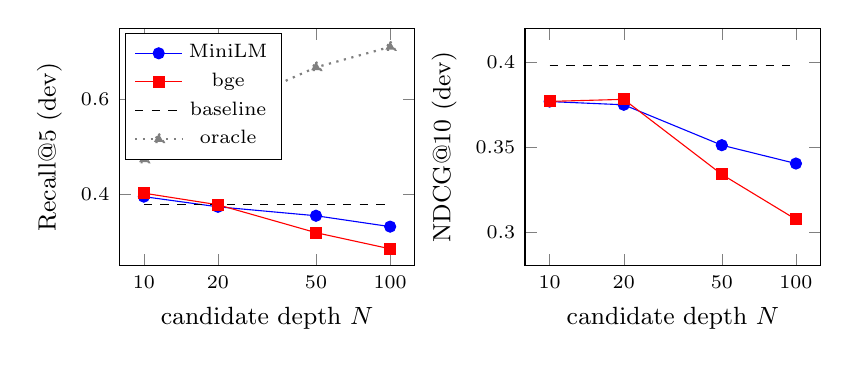
\begin{tikzpicture}
\begin{axis}[name=left, width=0.44\linewidth, height=4.6cm, xmode=log, log basis x=10,
  xtick={10,20,50,100}, xticklabels={10,20,50,100}, xlabel={candidate depth $N$},
  ylabel={Recall@5 (dev)}, ymin=0.25, ymax=0.75, legend style={font=\scriptsize, at={(0.02,0.98)}, anchor=north west},
  tick label style={font=\scriptsize}, label style={font=\small}]
\addplot[mark=*, blue] coordinates {(10,0.3957) (20,0.3743) (50,0.3555) (100,0.3326)};
\addplot[mark=square*, red] coordinates {(10,0.4030) (20,0.3786) (50,0.3199) (100,0.2859)};
\addplot[dashed, black, domain=10:100] {0.3795};
\addplot[dotted, thick, gray, mark=triangle*] coordinates {(10,0.4740) (20,0.5760) (50,0.6678) (100,0.7106)};
\legend{MiniLM, bge, baseline, oracle}
\end{axis}
\begin{axis}[at={(left.east)}, anchor=west, xshift=1.4cm, width=0.44\linewidth, height=4.6cm, xmode=log,
  xtick={10,20,50,100}, xticklabels={10,20,50,100}, xlabel={candidate depth $N$},
  ylabel={NDCG@10 (dev)}, ymin=0.28, ymax=0.42,
  tick label style={font=\scriptsize}, label style={font=\small}]
\addplot[mark=*, blue] coordinates {(10,0.3768) (20,0.3749) (50,0.3511) (100,0.3403)};
\addplot[mark=square*, red] coordinates {(10,0.3769) (20,0.3781) (50,0.3339) (100,0.3074)};
\addplot[dashed, black, domain=10:100] {0.3983};
\end{axis}
\end{tikzpicture}
\caption{Retrieval quality on dev (125 questions) after reranking the top-$N$ dense candidates. Dashed: baseline (no reranking). Dotted: oracle Recall@5, the best any reranker of the top $N$ could reach.}
\label{fig:quality}
\end{figure}

Figure~\ref{fig:quality} shows the main retrieval result. The oracle line rises from 0.47 to 0.71 as $N$ grows, so there is plenty of room to improve. Both rerankers instead \emph{fall} as $N$ grows, and the large model falls faster (bge: 0.40 at $N{=}10$ to 0.29 at $N{=}100$). At $N{=}10$ both are slightly above the baseline on Recall@5 (+1.6 and +2.4 points), but at every $N$ both are below the baseline on NDCG@10 and MRR@10. On practice the same pattern holds, except that even $N{=}10$ is below the baseline on Recall@5 (Appendix~\ref{app:sweeps}). The small dev gain at $N{=}10$ is therefore not a stable effect.

\subsection{Cost: latency grows with $N$ and with model size}

\begin{table}[h]
\caption{Reranking cost on dev (benchmark, no LLM calls): latency per query in ms, median (p95) over 5 repeats $\times$ 125 questions after warm-up; peak GPU memory; model load time (varies with file-system caching across runs).}
\label{tab:cost}
\centering\small
\setlength{\tabcolsep}{4pt}
\begin{tabular}{lrrrrrr}
\toprule
Model & $N{=}10$ & $N{=}20$ & $N{=}50$ & $N{=}100$ & Peak GPU mem. & Load time \\
\midrule
MiniLM (22M) & 32 (36) & 61 (67) & 113 (126) & 169 (194) & 359\,MB & 0.5--2.1\,s \\
bge (278M) & 111 (117) & 220 (228) & 402 (437) & 647 (742) & 1599\,MB & 3.9--31\,s \\
\bottomrule
\end{tabular}
\end{table}

Table~\ref{tab:cost} shows that latency grows almost linearly with $N$, because the cross-encoder needs one transformer pass per (question, record) pair. bge is 3.5--3.8$\times$ slower than MiniLM, in line with its $\sim$12$\times$ more parameters. Going from $N{=}10$ to $N{=}20$ doubles the time even though both fit in one batch of 32. So the cost per pair is not just GPU arithmetic: tokenisation on the CPU and padding to the longest pair in the batch probably matter too. In the full pipeline, reranking is small compared with generation. The median ELM call takes 4.4--4.9\,s, so reranking adds about 2--3\% to the post-ASR latency. In the full runs the measured \texttt{rerank\_ms} was higher than in the benchmark (median 96 vs 61\,ms for MiniLM, 140 vs 111\,ms for bge), probably because the encoder and the reranker compete for the CPU.

\subsection{Answer quality: no clear change}

\begin{table}[h]
\caption{End-to-end results on dev (125 questions, same cached transcripts, $k{=}5$). Retrieval metrics come from the sweep (same deterministic reranking). Judge = mean normalised score (0--1, higher is better); $\Delta$ = paired mean difference vs baseline, 95\% bootstrap CI and sign-flip $p$. Latencies are medians in ms; end-to-end excludes ASR.}
\label{tab:main}
\centering\small
\setlength{\tabcolsep}{3pt}
\resizebox{\linewidth}{!}{%
\begin{tabular}{lccccccccc}
\toprule
Config & R@5 & MRR@10 & NDCG@10 & Judge & $\Delta$ judge [95\% CI], $p$ & Zero scores & Rerank & Prompt chars & End-to-end \\
\midrule
Baseline & 0.380 & 0.460 & 0.398 & 0.314 & -- & 56 & -- & 4980 & 5050 \\
MiniLM $N{=}20$ & 0.374 & 0.428 & 0.375 & 0.305 & $-0.009$ [$-0.065$, $+0.048$], 0.78 & 59 & 96 & 6004 & 5116 \\
bge $N{=}10$ & 0.403 & 0.419 & 0.377 & 0.349 & $+0.035$ [$-0.021$, $+0.089$], 0.24 & 52 & 140 & 5362 & 4779 \\
\bottomrule
\end{tabular}}
\end{table}

Table~\ref{tab:main} gives the end-to-end comparison. Both confidence intervals include zero, so we cannot claim either reranker changes answer quality. The bge configuration is the best on every judge part (correctness 1.44 vs 1.32, grounding 1.52 vs 1.35, completeness 1.22 vs 1.10, each out of 4), but with 125 questions this difference is within noise. The end-to-end differences come from ELM network time (bge is the fastest despite longer prompts), not from reranking.

\subsection{Why reranking does not help here}
\label{sec:why}

\textbf{Does evidence quality drive answer quality?} Yes, and this is the clearest positive finding. We split the dev questions by whether reranking raised, lowered or kept Recall@5. With bge $N{=}10$, the 17 questions whose Recall@5 rose gained $+0.18$ in judge score on average (8 better, 1 worse), the 11 whose Recall@5 fell lost $0.05$, and the 97 unchanged ones moved by only $+0.02$. With MiniLM $N{=}20$ the pattern is the same ($+0.10$ for 19 up, $-0.17$ for 17 down). The correlation between the change in Recall@5 and the change in judge score is 0.22 (bge) and 0.28 (MiniLM). So the pipeline \emph{does} reward better evidence. The problem is that reranking improves the evidence for only 14--15\% of questions and makes it worse for 9--14\%, which cancels out.

\textbf{The rerankers demote correct first results.} The baseline has a relevant record at rank 1 for 47 dev questions (144 practice). After reranking, MiniLM $N{=}20$ keeps only 33 of these (111 on practice) and bge $N{=}10$ keeps only 28 (91). Both find some new rank-1 hits, but not enough to make up for the loss, which is why MRR@10 falls in every configuration. The supplied \texttt{enc\_a} encoder seems to be well matched to this corpus, while the rerankers are not.

\textbf{Domain mismatch, the most likely cause.} MiniLM was trained on MS MARCO web-search queries and bge on general data. Our records are long, informal finance-forum posts, and our questions are spoken and come through ASR. Cross-encoders are known to lose much of their advantage out of domain~\citep{thakur2021beir}. Two observations support this. (i) Quality falls as $N$ grows (Figure~\ref{fig:quality}): deeper candidates are mostly off-topic, and the more of them the reranker sees, the more often a plausible-looking but irrelevant post wins. (ii) The larger, more general bge model does \emph{worse} at large $N$ than the small one, so model capacity is not the bottleneck; matching training data is.

\textbf{Other explanations we checked.} \emph{Truncation:} 9.7\% (MiniLM) and 11.5\% (bge) of pairs exceed 512 tokens and lose their end. This can hide the relevant part of a long post, but it affects too few pairs to explain the large drop at $N{=}100$. \emph{ASR errors:} the transcripts are identical in all conditions, so ASR noise cannot explain the \emph{differences}, although it may hurt both systems equally. \emph{Prompt length (a confound):} the rerankers prefer longer records, so their prompts are 8\% (bge) and 21\% (MiniLM) longer. This raises ELM token cost and could itself change answers, so we cannot fully separate ``better records'' from ``longer records''. \emph{Judge and generation noise:} for the 5 questions where the reranker picked the same 5 records as the baseline (only reordered), 3 still got a different judge score. Scores therefore vary even when the evidence is the same, which is why paired tests and confidence intervals are needed.

\section{Discussion and conclusion}
\label{sec:conclusion}

For the ASR part, our hand-written kernels are correct and our small memory-bound kernels are fast (RoPE reaches 80\% of peak bandwidth), but the simple tiled GEMM is $4$--$9\times$ slower than cuBLAS and makes the whole model $3.1\times$ slower than PyTorch. Register tiling and vectorised loads in GEMM would be the next step, because GEMM is 84\% of the time.

For RAG, our evidence supports a precise but limited conclusion: \emph{on this corpus, an off-the-shelf cross-encoder in front of \texttt{enc\_a} costs 30--650\,ms, up to 1.6\,GB of GPU memory and 8--21\% longer prompts, and gives no measurable gain in answer quality.} The trade-off is poor because the rerankers do not reliably rank in-domain records better than the supplied encoder. Answers did get better when Recall@5 rose, so this conclusion would likely change with (a) a reranker fine-tuned on in-domain question--record pairs, or (b) combining the dense and reranker scores, so that the reranker can only move records the encoder already likes. Neither was tested.

\textbf{Limitations.} 125 dev questions give wide confidence intervals ($\pm$0.055). Each answer was judged once, and the same model generates and judges, which may bias the judge towards its own style~\citep{zheng2023judge}. All timings are from one GPU type, and the ELM latency depends on a shared network service. We chose $N$ on practice, so the two dev configurations are each model's best on practice, not on dev.

% References are excluded from the main-body page limit.
\bibliography{references}
\bibliographystyle{iclr2027_conference}

\appendix
\section{HW1 outputs (RTX 2080 Ti)}
\label{app:hw1}
\texttt{nvidia-smi -L}: \texttt{GPU 0: NVIDIA GeForce RTX 2080 Ti}. All rows below are from \texttt{make test} and \texttt{./run.sh --profile} run in the same session on that node.

{\tiny
\begin{verbatim}
Task 1 (RoPE)                          time        rate
tiny (2 x 3 tokens, Hq=3, Hk=1)  PASS  0.003 ms    0.5 GB/s ( 0% of peak)
odd sizes, partial rotation      PASS  0.003 ms    5.8 GB/s ( 1% of peak)
audio encoder (partial, 32/64)   PASS  0.031 ms  490.8 GB/s (80% of peak)
text decoder (GQA 16/4, full)    PASS  0.004 ms  310.5 GB/s (50% of peak)       -> ALL PASS
Task 2 (reductions)
rmsnorm, text decoder            PASS  0.006 ms  163.5 GB/s (27% of peak)
layernorm, audio encoder         PASS  0.040 ms  380.5 GB/s (62% of peak)
softmax, vocabulary row (59264)  PASS  0.126 ms    3.8 GB/s ( 1% of peak)
softmax, 64 x 4096               PASS  0.010 ms  217.7 GB/s (35% of peak)
(+7 small/edge cases: short rows, odd cols, +-100 inputs, all negative)  -> ALL PASS
Task 3 (tiled GEMM)                           ours        naive       cuBLAS (GFLOP/s)
decoder q_proj (64x2048x2048)        PASS  0.440 ms  1220         153         4663
decoder gate_proj (64x6144x2048)     PASS  1.205 ms  1337         162         6795
decoder down_proj (64x2048x6144)     PASS  1.212 ms  1329         196         8158
lm_head, last token (1x59264x2048)   PASS  2.005 ms   121         115          291
encoder q_proj (1500x1280x1280)      PASS  2.670 ms  1841         224        13047
encoder fc1 + GELU (1500x5120x1280)  PASS 14.267 ms  1378         225        12765
conv2 via im2col (1500x1280x3840)    PASS 10.214 ms  1444         225        13037
(+3 small/odd cases)                                              -> ALL PASS
Task 4 (attention)
several tiles, peaky scores          PASS  0.014 ms    16 GFLOP/s
text decoder (GQA 16/4, causal)      PASS  0.066 ms   255 GFLOP/s
audio encoder (20 heads, 1500)       PASS 11.416 ms  1009 GFLOP/s
(+5 small/causal/GQA cases)                                       -> ALL PASS

./run.sh --profile (all kernels ours)    ./run.sh --cuda none --profile (PyTorch)
linear     2757 calls  2875.0 ms 84.2%   linear     597.4 ms 41.6%
attention   396 calls   521.1 ms 15.3%   rope       433.3 ms 30.1%
rmsnorm     741 calls     6.1 ms  0.2%   attention  313.3 ms 21.8%
silu_mul    364 calls     3.3 ms  0.1%   rmsnorm     85.5 ms  5.9%
rope        396 calls     2.7 ms  0.1%   silu_mul     4.0 ms  0.3%
layernorm    65 calls     2.4 ms  0.1%   layernorm    2.6 ms  0.2%
softmax      13 calls     1.6 ms  0.0%   embedding    1.0 ms  0.1%
embedding    13 calls     1.2 ms  0.0%   im2col       0.3 ms  0.0%
im2col        2 calls     0.2 ms  0.0%   softmax      0.3 ms  0.0%
Time: 3283.1 ms (+/- 8.8) per transcription   Time: 1065.0 ms (+/- 0.2)
252.5 ms per token, peak GPU memory 8.56 GiB  81.9 ms per token, 8.88 GiB
Transcription: Concord returned to its place amidst the tents.  Accuracy: 100.0%  Status: PASS
\end{verbatim}
}

\section{Full reranking sweeps}
\label{app:sweeps}

\begin{table}[h]
\caption{Retrieval sweep on both splits (Recall@5 / NDCG@10 / MRR@10). Recall@100 is unchanged by construction (practice 0.770, dev 0.724).}
\centering\small
\resizebox{\linewidth}{!}{%
\begin{tabular}{lccc}
\toprule
Config & Practice (350) & Dev (125) & Median rerank ms (dev) \\
\midrule
Baseline & 0.421 / 0.420 / 0.489 & 0.380 / 0.398 / 0.460 & -- \\
MiniLM $N{=}10$ & 0.404 / 0.405 / 0.464 & 0.396 / 0.377 / 0.424 & 32 \\
MiniLM $N{=}20$ & 0.411 / 0.414 / 0.471 & 0.374 / 0.375 / 0.428 & 61 \\
MiniLM $N{=}50$ & 0.399 / 0.399 / 0.454 & 0.356 / 0.351 / 0.412 & 112 \\
MiniLM $N{=}100$ & 0.388 / 0.395 / 0.453 & 0.333 / 0.340 / 0.400 & 167 \\
bge $N{=}10$ & 0.392 / 0.382 / 0.428 & 0.403 / 0.377 / 0.419 & 108 \\
bge $N{=}20$ & 0.377 / 0.371 / 0.408 & 0.379 / 0.378 / 0.426 & 215 \\
bge $N{=}50$ & 0.351 / 0.340 / 0.383 & 0.320 / 0.334 / 0.396 & 398 \\
bge $N{=}100$ & 0.327 / 0.313 / 0.353 & 0.286 / 0.307 / 0.359 & 643 \\
\midrule
Oracle R@5 ($N$ = 10/20/50/100) & 0.477 / 0.575 / 0.679 / 0.764 & 0.474 / 0.576 / 0.668 / 0.711 & \\
\bottomrule
\end{tabular}}
\end{table}

Practice baseline answer quality: judge score 0.335 over 350 questions (20 judgements, 5.7\%, used the JSON fallback). Throughput in the benchmark rises with $N$ (MiniLM 342 to 593 pairs/s; bge 99 to 155 pairs/s) because larger $N$ fills the batches of 32 better.

% Keep this line unchanged.
\newpage

% Academic integrity is an underlying principle of research and academic practice.
% All submitted work is expected to be your own, including any material you have
% generated yourself with the assistance of AI tools such as ELM, ChatGPT,
% Bing Chat, Claude, Google Gemini, or any other automated assistance.
% For all such material you must make prominent explicit acknowledgement and
% explain clearly what you have done in this section.
% This includes using AI to directly generate text, code, figures or similar
% or to complete other tasks. In all cases, you remain entirely responsible
% for the material you produce.
\section*{AI declaration}
We used Claude Code (Anthropic, Claude Opus model) as an assistant throughout this coursework. Specifically:
(1) \textbf{HW1 kernels:} to explain CUDA concepts (warp shuffles, tiling, online softmax) and to help debug our own kernel code; to check our numbers and help word our answers to the task-guide questions.
(2) \textbf{RAG investigation:} it wrote the fallback parser for malformed judge JSON, and it wrote the reranking code (\texttt{rag/extensions/reranker.py}, \texttt{bench\_rerank.py}, \texttt{rag/scripts/evaluate\_rerank.py}, the changes to \texttt{rag.py} and \texttt{generate\_answers.py}, and \texttt{rag/tests/test\_rerank.py}) from a plan we discussed and agreed with it. It also helped plan the experiment, gave the cluster commands, and wrote the script for the paired statistical analysis.
(3) \textbf{Report:} it drafted the text, tables and figures of this report from our result files; we reviewed and edited them.
We ran every experiment on the cluster ourselves, checked the reported numbers against the output files, and take full responsibility for all the content.
We also used the University ELM service (EuroLLM-22B-Instruct) as part of the system itself, as the answer generator and judge, as the coursework requires.

% Please put the information of your group here without changing the format.
% This page will be deleted when the report is distributed for reviewing.
\section*{Group information}
Group ID: XXX

Information of group member A:
\begin{itemize}
    \item Name: John Doe
    \item UUN: sXXXXXXX
\end{itemize}

% Keep this COMMENTED OUT, unless there is more than one member.
Information of group member B:
\begin{itemize}
    \item Name: John Doe
    \item UUN: sXXXXXXX
\end{itemize}

% Keep this COMMENTED OUT, unless there is more than one member and you feel like
% it is necessary to point out the contribution. Please notice that members from
% the same group technically receive the same score for the report, regardless of
% the contribution.
% \section*{Contribution}

\end{document}
